\documentclass{homework}
\usepackage{multicol}
\usepackage[dvipsnames]{xcolor}


\title{Tarea 1}
\date{2019-08-30}
\gdate{2do Semestre 2019}
\author{Nicholas Mc-Donnell}
\course{Ecuaciones Diferenciales Ordinarias - MAT2500}


\begin{document}
\maketitle
\thanks{Maximiliano Norbu, Agustín Oyarce, Camilo Sánchez, Benjamín Cortez, Felipe Guzmán}
\pagenumbering{roman}
\newpage
\tableofcontents
\newpage
\pagenumbering{arabic}
\begin{prob}
    Transforme las siguientes EDOs en sistemas autónomos de primer orden:
    \begin{enumerate}
        \item \(\ddot{x}+t\sin(\dot{x})=x\).
        \item \(\ddot{x}=-y,\ddot{y}=x\).
    \end{enumerate}
\end{prob}

\begin{sol}
    Se toman los siguientes sistemas autónomos de primer orden, y se nota que son equivalentes a los correspondientes:
    \begin{enumerate}
        \item \(\dot{t}=1\), \(z=\dot{x}\), \(\dot{z}+t\sin(z)=x\)
        \item \(w=\dot{x}\), \(y=-\dot{w}\), \(x=\dot{z}\), \(z=\dot{y}\)
    \end{enumerate}
\end{sol}

\begin{prob}
    Encuentre soluciones a las siguientes EDOs:
    \begin{enumerate}
        \item \(\dot{x}=x(1-x)\)
        \item \(\dot{x}=\sin(t)\exp(x)\)
    \end{enumerate}
\end{prob}

\begin{sol}
    \begin{enumerate}
        \item Notemos que \(x(t)\equiv0\) y \(x(t)\equiv1\) son soluciones, por lo que se puede asumir que \(x\neq1\) y \(x\neq0\) localmente. Usando un poco de álgebra se llega a la siguiente ecuación:
        \begin{equation*}
            \frac{\dot{x}}{x(1-x)}=1
        \end{equation*}
        La cual se puede integrar, quedando lo siguiente:
        \begin{equation*}
            \int_{x(t_0)}^{x(t)}\frac{\d{x}}{x(1-x)}=\int_{t_0}^t\d{s}
        \end{equation*}
        Se nota que \(\frac1{x(1-x)}=\frac1x+\frac1{1-x}\), por lo que la ecuación anterior se ve de la siguiente forma:
        \begin{equation*}
            \ln(x(t))-\ln(x(t_0))-\ln(1-x(t))+\ln(1-x(t_0))=t-t_0
        \end{equation*}
        Con lo que se ve que
        \begin{equation*}
            \frac{x(t)}{x(t_0)}\cdot\frac{1-x(t_0)}{1-x(t)}=\exp(t-t_0)
        \end{equation*}
        Y por un poco de álgebra se tiene lo siguiente:
        \begin{equation*}
            x(t)=\dfrac{\frac{x(t_0)}{1-x(t_0)}\exp(t-t_0)}{1+\frac{x(t_0)}{1-x(t_0)}\exp(t-t_0)}
        \end{equation*}
        La cual es una solución local.
        \item Se nota que la EDO es equivalente a la siguiente:
        \begin{equation*}
            \dot{x}\exp(-x)=\sin(t)
        \end{equation*}
        Por lo que se puede integrar, consiguiendo lo siguiente:
        \begin{equation*}
            \int_{x(t_0)}^{x(t)}\exp(-x)\d{x}=\int_{t_0}^t\sin(s)\d{s}
        \end{equation*}
        Solucionando las integrales y haciendo un poco de álgebra se tiene que:
        \begin{equation*}
            x(t)=-\ln(\cos(t)-\cos(t_0)+\exp(-x(t_0)))
        \end{equation*}
        Lo cual nos da una solución local.
    \end{enumerate}
\end{sol}

\begin{prob}
    Encuentre soluciones a las siguientes EDOs
    \begin{enumerate}
        \item \(\dot{x}=\frac{3x-2t}{t}\)
        \item \(y'=y^2-\frac{y}{x}-\frac1{x^2}\)
        \item \(y'=\frac{y}{x}-\tan({\frac{y}{x}})\)
    \end{enumerate}
\end{prob}

\begin{sol}
    \begin{enumerate}
        \item La EDO correspondiente se puede escribir de la siguiente manera\footnote{Recordando que \(t\neq0\)}:
        \begin{equation*}
            \dot{x}-\frac{3x}t=-2
        \end{equation*}
        Tomando el factor integrante \(\exp\paren{\int_{t_0}^t-3/t\d{t}}\), se llega a la siguiente igualdad:
        \begin{equation*}
            \paren{x\exp\paren{\int_{t_0}^t-3/s\d{s}}}'=-2\exp\paren{\int_{t_0}^t-3/s\d{s}}
        \end{equation*}
        Desarrollando el factor integrante e integrando en ambos lados se consigue lo siguiente:
        \begin{equation*}
            x(t)\cdot\paren{\frac{t_0}{t}}^3-x(t_0)=2t_0^3\paren{\frac1{t^4}-\frac1{t_0^4}}
        \end{equation*}
        Con lo que se ve que las soluciones son de la siguiente forma:
        \begin{equation*}
            x(t)=x(t_0)\cdot\paren{\frac{t}{t_0}}^3+2\paren{\frac1t-\frac{t^3}{t_0^4}}
        \end{equation*}
        Consiguiendo lo pedido.
        \item Para esta EDO se nota que la sustitución de Ricatti funciona, por lo que se necesita una solución particular. Notamos que \(y(x)=\frac1x\) es una solución particular\footnote{\(y'=-\frac1{x^2}=\frac1{x^2}-\frac1x\cdot\frac1x-\frac1{x^2}=y^2-\frac{y}x-\frac1{x^2}\)}, por lo que se usa la sustitución \(u=\frac1{y-\frac1x}\) y algo de álgebra para llegar a la siguiente EDO:
        \begin{equation*}
            u'+\frac{u}x=-1
        \end{equation*}
        La cual se puede solucionar multiplicando por el factor integrante:
        \begin{equation*}
            \paren{u\exp\paren{\int_{x_0}^x\frac1s\d{s}}}'=-\exp\paren{\int_{x_0}^x\frac1s\d{s}}
        \end{equation*}
        Ahora, integrando de nuevo y solucionando el factor integrante se llega a lo siguiente:
        \begin{equation*}
            u(x)\cdot\frac{x}{x_0}-u(x_0)=\frac{x}{x_0}-1
        \end{equation*}
        Con lo que tenemos la forma general de \(u(x)\):
        \begin{equation*}
            u(x)=\frac{x_0}xu(x_0)-\frac{x_0}x+1
        \end{equation*}
        Deshaciendo la sustitución se llega a lo siguiente:
        \begin{equation*}
            y(x)=\frac1x+\frac1{\frac{x_0}xu(x_0)-\frac{x_0}x+1}
        \end{equation*}
        Lo que nos da la forma general de una solución.
        \item Se ve que si se usa la sustitución \(u=\frac{y}{x}\), esto nos simplifica la EDO a lo siguiente:
        \begin{equation*}
            u'x+u=u-\tan(u)
        \end{equation*}
        Si es que \(u=0\), la función idénticamente cero es solución, por lo que se verán soluciones localmente no cero. Con esto se puede resolver la EDO escribiéndola de la siguiente forma:
        \begin{equation*}
            \frac{u'}{\tan(u)}=-\frac1x
        \end{equation*}
        Esto se puede integrar, y reordenar algebraicamente para conseguir esto:
        \begin{equation*}
            u(x)=\arcsin\paren{\frac{x_0}x\sin(u(x_0))}
        \end{equation*}
        Deshaciendo la sustitución, se consigue lo siguiente:
        \begin{equation*}
            y(x)=x\arcsin\paren{\frac{x_0}x\sin\paren{\frac{y(x_0)}{x_0}}}
        \end{equation*}
        Donde \(x\neq0\) e \(y(x_0)\neq0\), con lo que tenemos una solución local.
    \end{enumerate}
\end{sol}

\begin{prob}
    Sean \(\tau>0\) y \(\gamma>0\) constantes. Considere
    \[\dot{x}=\gamma\sqrt{\abs{x}}-\tau x,\quad x(0)=x_0\]
    \begin{enumerate}
        \item Resuelva el problema. (\textit{Sugerencia}: La EDO es de tipo Bernoulli)
        \item Analice la unicidad de la solución, y determine el intervalo máximo de definición. Si hay falla de unicidad, explique porqué esto no contradice el teorema de Picard-Lindelöf.
        \item Analice el comportamiento a largo plazo, \(t\rightarrow\infty\), cuando \(x_0>0\).
    \end{enumerate}
\end{prob}

\begin{sol}
    \begin{enumerate}
        \item Se nota que la EDO es autónoma, por lo que al solucionar el problema localmente para \(t=0\), se soluciona localmente para cualquier \(t_0\). Dado esto que la función \(x(t)\equiv0\) es solución si \(x_0=0\). También se nota que \(f\) es lipschitz con respecto a \(x\) para todo \(x\neq0\), y al ser autónoma es uniformemente continua con respecto \(t\), por lo que dado una condición inicial \(x_0\neq0\) se tiene solución única, por el teorema de Picard-Lindelöf. Sea \(x_0>0\) entonces localmente se puede hacer la sustitución \(x=y^2\), lo que nos da la siguiente EDO:
        \begin{equation*}
            \dot{y}=\frac\gamma2-y\frac\tau2 
        \end{equation*}
        Una EDO separable, por lo que integrando directamente y reordenando se llega a:
        \begin{equation*}
            y(t)=\frac\gamma\tau-\paren{\frac\gamma\tau-x_0^2}\exp\paren{-\frac{\tau\cdot t}2}
        \end{equation*}
        Se recuerda la sustitución que se uso, y se deshace, pero se considera que \(x(0)=x_0>0\)\footnote{Al usar \(x=y^2\) se pierde la noción de positividad, por lo que al deshacer la sustitución, se necesita considerarla.}. Con eso se llega a la presente solución:
        \begin{equation*}
            x(t)=\sqrt{\frac\gamma\tau-\paren{\frac\gamma\tau-x_0^2}\exp\paren{-\frac{\tau\cdot t}2}}
        \end{equation*}
        Similarmente para \(x_0<0\), se tiene la siguiente solución:\begin{equation*}
            x(t)=\sqrt{-\frac\gamma\tau+\paren{\frac\gamma\tau+x_0^2}\exp\paren{-\frac{\tau\cdot t}2}}
        \end{equation*}
        \item Como la EDO no es lipschitz cerca de \(0\), se tiene que cada vez que una solución tenga una intersección con el \(0\) esta se puede extender de variadas formas, por lo que no hay unicidad de solución, esto no contradice Picard-Lindelöf ya que no es lipschitz cerca de \(0\). Para ver el intervalo máximo de definición hay notar que dado \(x_0>0\), se necesita que \(y(t)\geq0\), lo cual se cumple para todo \(T_-<t\), donde \(T_-<0\) es un valor dependiente de \(x_0,\gamma\) y \(\tau\). Similarmente, para \(x_0<0\) se tiene que \(t<T_+\), donde \(T_+>0\) es un valor que depende de \(x_0,\gamma\) y \(\tau\).
        \item Como se vio anteriormente si \(x_0>0\), \(x(t)\) esta bien definida para todo \(t\) positivo, luego, viendo las soluciones es claro que cuando \(t\rightarrow\infty\) entonces \(x(t)\rightarrow\sqrt{\frac\gamma\tau}\).
    \end{enumerate}
\end{sol}
\begin{prob}
    Sea \(J\subseteq\set{R}\) un intervalo abierto. Suponga que el problema de valor inicial
    \[\begin{cases}
            \dot{x}=f(t,x) & (t,x)\in J\times\set{R},\quad f\in C(J\times\set{R}) \\
            x(t_0)=x_0
        \end{cases}\]
    tiene una solución \(C^1\) definida localmente en tiempo para todos datos iniciales \((t_0,x_0)\in J\times\set{R}\). Demuestre que si el intervalo máximo de definición de una solución \(x(t)\) es \((T_-,T_+)\subseteq J\), entonces \(\lim_{t\downarrow T_-}\abs{x(t)}=\infty\) y \(\lim_{t\uparrow T_+}\abs{x(t)}=\infty\). (\textit{Sugerencia}: Argumente por contradicción. Primero demuestre que si hay dos sucesiones \(\{a_i\}\) y \(\{b_j\}\) con \(a_i\uparrow T_+\) y \(b_j\uparrow T_+\) tales que \(x(a_i)\rightarrow x_1\) y \(x(b_j)\rightarrow x_2\), entonces \(x_1=x_2\). Úselo para probar que \(x(t)\) se puede extender como una solución después del momento \(T_+\)).
\end{prob}

\begin{sol}
    Se nota que la demostración para ambos límites es equivalente, por lo que se toma el caso de \(t\uparrow T_+\), y se asume que el límite no es infinito. Ahora sean, \(\{a_i\}\) y \(\{b_j\}\) sucesiones tal que \(a_i\uparrow T_+\) y \(b_j\uparrow T_+\), y además \(x(a_i)\rightarrow x_1\) y \(x(b_j)\rightarrow x_2\). Si \(x_1\neq x_2\), sea \(\varepsilon_n=\frac1n\), se pueden encontrar \(a_i,a_k\) y \(b_j\), tal que \(a_i<b_j<a_k\) y \(x_1-x(a_k)<x_2-x(b_j)<x_1-x(a_i)<\varepsilon_n\), ahora por TVM existen \(t_{n,1}\in(a_i,b_j)\) y \(t_{n,2}\in(b_j,a_k)\) tal que \(\frac{x(b_j)-x(a_i)}{b_j-a_i}=\dot{x}(t_{n,1})\) y \(\frac{x(a_k)-x(b_j)}{a_k-b_j}=\dot{x}(t_{n,2})\). Se nota que desde un \(n\) suficientemente grande se tiene que \(\dot{x}(t_{n,2})>0\) y \(\dot{x}(t_{n,1})<0\), o \(\dot{x}(t_{n,2})<0\) y \(\dot{x}(t_{n,1})>0\), pero la diferencia entre \(t_{n,1}\) y \(t_{n,2}\) disminuye para un \(n\) cada más grande, lo implicaría que \(\dot{x}\) no es continua cerca de \(T_+\), pero \(x\) es \(C^1\). Por ende, \(x_1=x_2\), con lo que para todo sucesión \(c_k\uparrow T_+\) se tiene que \(\lim_{k\rightarrow\infty}x(c_k)=x_1\), por lo que se puede extender \(x(t)\) a \(T_+\), lo que contradice que que el intervalo máximo es \((T_-,T_+)\).
\end{sol}

\begin{prob}
    Considere el problema de valor inicial
    \[\begin{cases}
            \dot{x}=x^3-\exp(t^2)x^2 & (t,x)\in[0,\infty)\times\set{R} \\
            x(0)=\xi
        \end{cases}\]\
    \begin{enumerate}
        \item Identifique y dibuje las 0-isoclinas de la ecuación.
        \item Demuestre que para \(\xi\in[0,1]\), la solución \(x(t)\) está definida para todos \(t\geq0\), y que \(\lim_{t\rightarrow\infty}x(t)=0\).
        \item Pruebe que cuando \(\xi\geq K\) es suficientemente grande, \(x(t)\) explota en tiempo finito. (\textit{Sugerencia}: Construya una subsolución de la forma \(y(t)=\exp(t^2)g(t)\) que explota en tiempo finito).
    \end{enumerate}
\end{prob}

\begin{sol}
    \begin{enumerate}
        \item Las 0-isoclinas se calculan de la siguiente manera:
        \begin{equation*}
            x^2(x-\exp(t^2))=0
        \end{equation*}
        Con lo que se ven dos 0-isoclinas:
        \begin{center}
            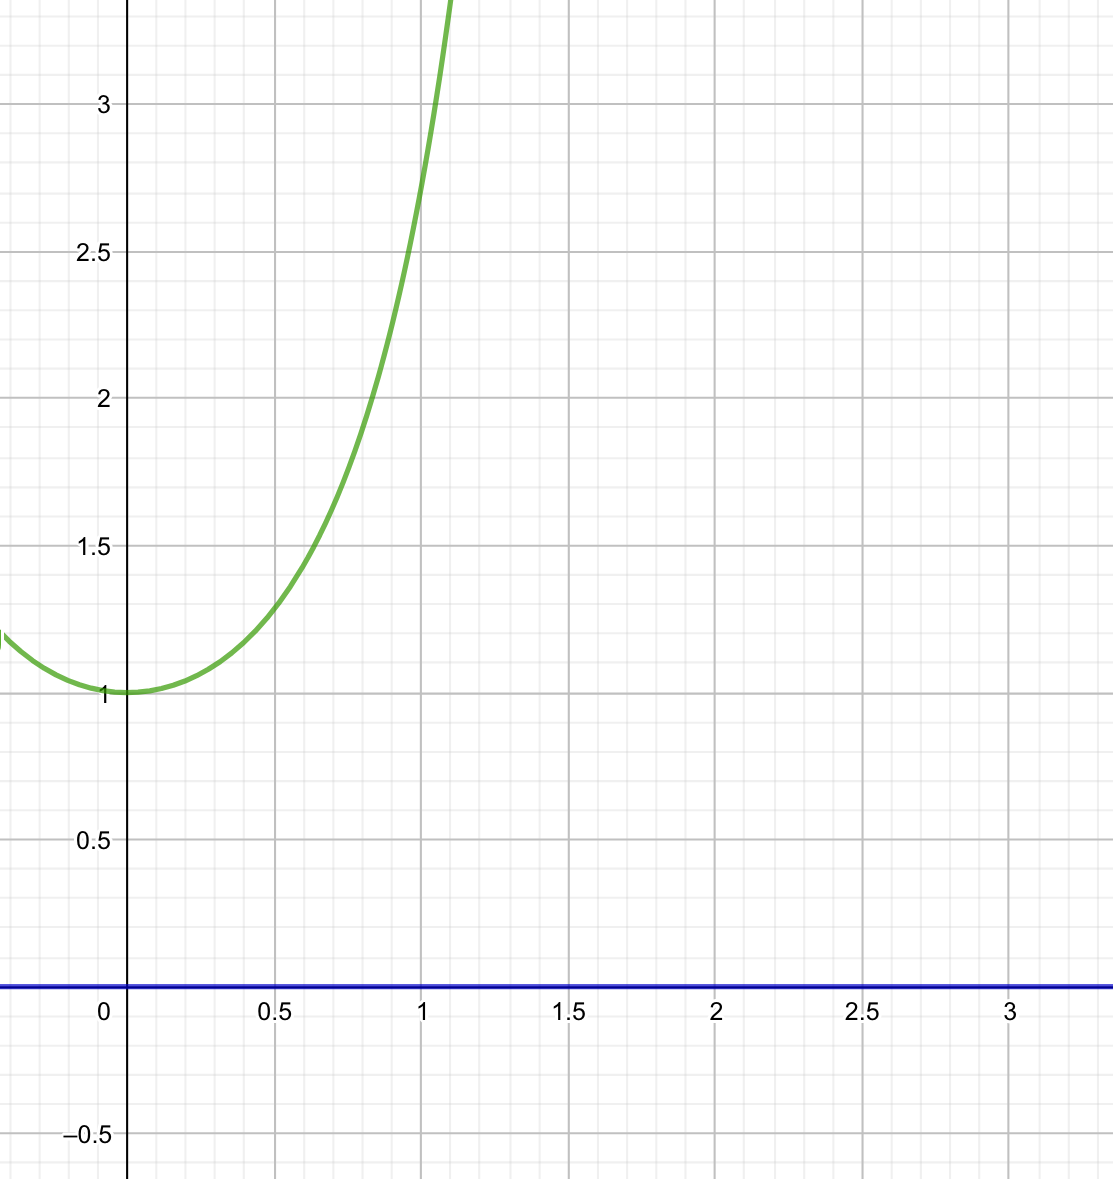
\includegraphics{Isoclines.png}
        \end{center}
        Donde \(\textcolor{OliveGreen}{f(t)=\exp(t^2)}\) y \(\textcolor{blue}{g(t)=0}\)
        \item Dado la condición inicial es suficiente demostrar que \(x(t)\) es decreciente para que este definida para todo \(t\geq0\). Sea \(x\in[0,1]\), entonces la siguiente desigualdad se cumple:
        \begin{equation*}
            \dot{x}=x^3-\exp(t^2)x^2=x^2(x-\exp(t^2))\leq1-\exp(t^2)\leq0
        \end{equation*}
        Por lo que para \(x\in[0,1]\) \(x(t)\) es decreciente. Ahora, como \(x(t)\) es decreciente y acotada inferiormente\footnote{Por la solución y 0-isoclina \(x(t)\equiv0\)} se tiene que existe el límite \(lim_{t\rightarrow\infty}x(t)\), se llamará \(k\) a este límite. Si \(k=0\) se tiene lo pedido, por lo que se considerará \(k>0\)
        \item Para demostrar esto, sea \(y(t)=\exp(t^2)\frac1{\paren{x-1/2}^2}\), esta es una subsolución que explota en tiempo finito, por lo que se tiene lo pedido.
    \end{enumerate}
\end{sol}

\begin{prob}
    Sea \(C\subseteq X\) un subconjunto cerrado del espacio de Banach \(X\). Suponga que para la función \(K:C\rightarrow C\), su \(n\)-ésima iteración \(K^n:C\rightarrow C\) es una contracción. Demuestre que \(K\) tiene un único punto fijo en \(C\).
\end{prob}

\begin{sol}
    Por pto. fijo de Banach, se tiene que \(K^n\) tiene un pto. fijo único, el cual se denotará como \(\overline{x}\), luego
    \begin{align*}
        K^n(K(\overline{x}))&=K^{n+1}(\overline{x})\\
        &=K(K^n(\overline{x}))\\
        &=K(\overline{x})\quad\text{ya que \(\overline{x}\) es pto. fijo de \(K^n\)}
    \end{align*}
    Entonces \(K(\overline{x})\) es pto. fijo de \(K^n\), pero este es único, por lo que \(K(\overline{x})=\overline{x}\). Lo que significa que \(K\) tiene un pto. fijo.
\end{sol}

\begin{prob}
    (La Desigualdad de Gronwall): Suponga que \(\psi(t)\) satisface
    \[\psi(t)\leq\alpha(t)+\int_0^t\beta(s)\psi(s)\d{s},\quad t\in[0,T]\]
    con \(\alpha(t)\in\set{R}\) y \(\beta(t)\geq0\). Entonces
    \[\psi(t)\leq\alpha(t)+\int_0^t\alpha(s)\beta(s)\exp\paren{\int_s^t\beta(r)\d{r}}\d{s},\quad t\in[0,T]\]
    Es más, si además \(\alpha(s)\leq\alpha(t)\) para \(s\leq t\), entonces
    \[\psi(t)\leq\alpha(t)\exp\paren{\int_0^t\beta(s)\d{s}},\quad t\in[0,T].\]\\
    Demuestre la última desigualdad.
\end{prob}

\begin{sol}

\end{sol}
\end{document}